\chapter{Metodologia}

Nessa seção listaremos os fundamentos teórico-aplicados utilizados na análise
dos synsets, bem como elucidaremos as estratégias e convenções dessa análise.
Esses dois aspectos da metodologia do projeto permitem o estabelecimento de um
estilo padrão para os synsets da WordNet.Br. Também discutiremos a
implementação do Git~\cite{git}, software que foi selecionado para otimizar o
armazenamento e o gerenciamento dos diferentes tipos de arquivo que são gerados
na execução das atividades de construção da WordNet.Br.

\section{Metodologia de base}

Antes que qualquer análise de synsets seja feita, é necessário compreender os
aspectos teóricos por trás da WordNet de Princeton (doravante WN.Pr), produzida
para o inglês norte-americano, os pressupostos para o alinhamento de wordnets e
as particularidades da WordNet.Br (doravante WN.Br). Essa necessidade foi
suprida com o estudo dos textos da Bibliografia Básica.

Destacamos alguns textos fundamentais, como~\citeonline{fellbaum}, que descreve
minuciosamente a WN.Pr, e~\citeonline{vossen}, uma edição especial do periódico
\en{\textit{Computers and the Humanities}}, que discute as dificuldades e
estratégias na construção da EuroWordNet, uma mega-WordNet que associa
diferentes wordnets em construção para as línguas da União Européia. Incluímos
nessa lista~\citeonline{riemer}, que fornece o embasamento teórico que precedeu
àquele dos textos acima, discutindo teorias e conceitos da semântica (grasso e
lexical) que se provaram bastante úteis na compreensão das wordnets, em
especial o capítulo~8.

\section{Estratégias de execução}

De acordo com os fundamentos teóricos fornecidos pela Bibliografia Básica, para
cada synset selecionado da base da WN.Br, após análise léxico-semântica,
propõe-se uma glosa.

A metodologia aplicada neste primeiro mês de pesquisa apresentou grande
eficiência, o que diminui a probabilidades de que algum procedimento seja
alterado até julho.

Procedimentos:
	
\begin{enumerate}
  \item Iniciam-se os seguintes aplicativos:

    \begin{enumerate}[a.]
      \item \texttt{06artifact(11256).doc};
      \item Arquivo modelo para posterior indexação (\texttt{.txt});
      \item WordNet 2.0;
      \item Editor da WordNet.Br;
      \item Dicionários de inglês/inglês e inglês/português;
      \item Navegador de internet com acesso ao córpus (\nilc) e à
        ferramentas de busca (Google, AltaVista, Yahoo).
    \end{enumerate}

  \item\label{selecao_synset} Seleciona-se o synset do inglês que dará origem à
    análise ou construção do synset do português na lista de synsets do
    tipo~\texttt{06artifact(11256).doc} e localiza-se esse synset na base da
    WN.Pr; todo seu conteúdo (o synset e todas as informações associadas a ele,
    incluindo todos os seus hiperônimos) é copiado para o arquivo modelo em
    \texttt{.txt}.

  \item\label{analise_synset} Copia-se o synset do português semanticamente
    equivalente ao inglês, se ele já existir na base da WN.Br, para o arquivo
    referido em~\ref{selecao_synset}, analisando-o quanto à sua boa-formação
    ortográfica e semântico-conceitual (esta análise consiste em:  ampliar ou
    reduzir o synset, segmentá-lo em dois ou mais synsets ou excluí-lo da base
    do português); caso não haja um synset equivalente na base do português,
    constrói-se um novo synset que se alinhe conceitualmente ao synset do
    inglês referido em~\ref{selecao_synset}, ou seja, procura-se construir o
    synset português cujas unidades lexicais sejam traduções das unidades
    lexicais do synset do inglês.

  \item Durante os procedimentos em~\ref{analise_synset}, observa-se qual
    destas análises que, previstas em~\citeonline{vossenetal}, será a mais
    apropriada para especificar o alinhamento conceitual que resulta da
    análise: alinhamento por \eqsyn, por \eqnsyn, por \eqhypo\ ou por \eqhyper.

  \item Cria-se a glosa para o synset do português em construçao, com base na
    glosa já existente para o synset do inglês, quando esta já estiver
    especificada no synset do inglês.

  \item Para cada unidade lexical que constitui o synset do português,
    selecionam-se frases-exemplo em corpus. As frases localizada no corpus do
    Núcleo Interinstitucional de Linguística Computacional~\cite{nilc} têm
    prioridade sobre as frases localizadas pelas ferramentas de busca da web;
    usa-se o critério de maior frequência de ocorrência da unidade lexical em
    corpora para decidir a seleção das frases-exemplo; quando a frase é selecionada
  na web, sinaliza-se o fato, acrescentando-se ``\texttt{I]}'' (``proveniente da
  Internet'') a unidade lexical da frase que corresponde à unidade lexical do
  synset.

\item Define-se a chave do synset, que é a unidade lexical pertencente a ele e
  que é a mais frequente na busca em corpus ou a intuitivamente mais usada.

\item Conclui-se a análise e nomeia-se o arquivo segundo este padrão:

  \begin{center}
    \texttt{<n\textordmasculine\_na\_Base\_WNBr>.<ILI>.<tipo\_semântico>.
    <chave>.void|md|cr.HYPER|HYPO|NEAR|void>}
  \end{center}

\end{enumerate}

\section{Estratégia de gerenciamento dos arquivos}

% Aqui vão as coisas sobre o Git. Primeiro, usar o que está no resumo da
% apresentação do~\textsc{cic}. Isso deve introduzir o Git, sua motivação e
% uso, e brevemente sua história. Depois, devo discutir a abertura do projeto
% (transferido de um servidor privado a um servidor particular, \en{wording}
% que o Bento indicou). Finalmente, devo descrever os passos para utilizar o
% GitHub.  Talvez umas imagens no Windows, talvez algo mais técnico no linux,
% talvez ambos. Também posso discutir com o Bento que essas instruções podem
% mudar com o tempo, então seria muito mais interessante dar um link para o
% artigo no GitHub que descreve a instalação no Windows, OS~X e GNU\slash
% Linux.  Acredito, pessoalmente, que essa deve ser a melhor solução.
% 
% Comentar, aqui ou elsewhere, que o Git será apresentado no~\textsc{cic}.

A dimensão do desafio que é gerenciar a base de arquivos da~\wnbr\ pode ser
apreciada considerando-se que, entre~2010 e~2012, produzidos e revistos certa
de~4100 arquivos, correspondendo ao mesmo número de synsets produzidos e
alinhados. Cinco bolsistas de~\textsc{ic} supervisionados pelo coordenador
estiveram envolvidos nas tarefas, que significaram a exploração de diferentes
análises até a escolha final de cada synset considerado ideal para configurar
na base da~\wnbr; análises cujos históricos foram documentados para que toda e
qualquer decisão analítica pudesse ser recuperada, revista e atualizada.

A solução em teste para o desafio é a adoção do~Git, um sistema de controle de
versões de arquivos~\cite{chacon}, que deve viabilizar:

\begin{enumerate}
  \item O controle do histórico da construção e do alinhamento de synsets (Que
    análise foi feita? Quem a fez? Quando?);
  \item O registro de análises distintas para o mesmo synset, resultando em
    alinhamentos diferentes;
  \item O acesso, via Internet, a todos os arquivos gerados pelos
    desenvolvedores do projeto, pois cada desenvolvedor pode copiar todos os
    arquivos da base da \wnbr\ (no servidor) para a sua máquina local durante o
    seu trabalho, utilizar aqueles que são relevantes para as suas análises sem
    interferir na integridade dos mesmos, pois trabalha com uma cópia e seu
    acesso é restrito no servidor;
  \item A marcação e o resgate de uma versão do arquivo que registra o synset e
    o seu alinhamento considerador ideais;
  \item A consolidação da base da~\wnbr.
\end{enumerate}

Um Sistema de Controle de Versões~(SCV) resolve todos esses problemas,
permitindo ao usuário reverter seus arquivos a um estado anterior, reverter o
projeto inteiro a um estado anterior, comparar as mudanças ao longo do tempo,
ver quem foi o último a modificar os arquivos, e recuperar arquivos que foram
comprometidos ou deletados por acidente\footnote{\citeonline{chacon}:
\url{http://git-scm.com/book/en/Getting-Started-About-Version-Control}}.

A escolha do sistema de controle de versões~Git foi motivada por ser rápido,
estável, possuir todas as características apontadas acima e por sua licença de
software livre\footnote{\url{https://github.com/git/git/blob/master/COPYING}}.
Prova de que o~Git é capaz de gerenciar a base da~\wnbr\ é sua história. O
programa foi criado, originalmente, para gerenciar as mudanças no~Linux,
projeto para o qual mais de~7800 pessoas e quase~800 empresas já
contribuíram~\cite[p.~1]{corbetetal}.

Durante reuniões no final de~2010 e início de~2011, foram discutidos os
detalhes iniciais para a implementação do Git~\cite[p.~4]{beraldo11}. O Git foi
implementado e testado, usando um servidor cedido pelo~\nilc, no~\icmc\
(Instituto de Ciências Matemáticas e Computação) da \usp\ de São Carlos. Em
reunião no início do mês de~agosto, foi decidido que o repositório
da~WordNet.Br será movido do atual servidor de acesso privado no~\nilc\ para o
servidor de acesso público no~GitHub\footnote{\url{https://github.com/}}. Esse
movimento busca promover a divulgação do projeto e dos resultados obtidos até o
momento, bem como promover a comunicação entre os pesquisadores e demais
interessados. A figura~\ref{github:repositorio} apresenta a interface de um
repositório configurado no~GitHub.

%% Imagem da interface geral de um repositório no GitHub
\begin{figure}[h]
  \centering
  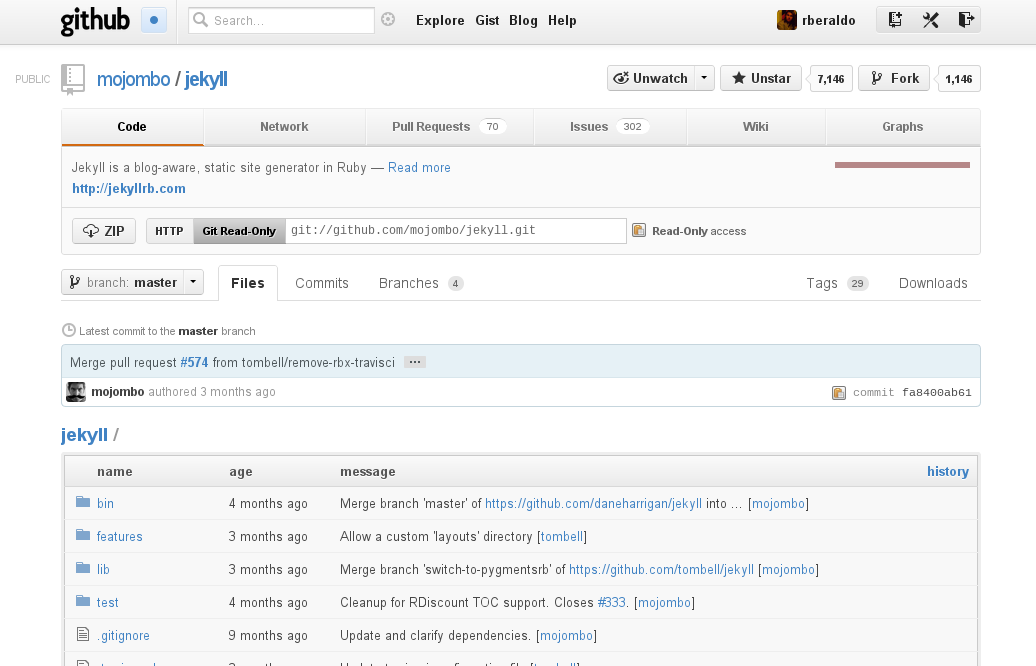
\includegraphics[width=.9\textwidth]{img/repositorio.png}
  \caption{A interface de um repositório no GitHub}
  \label{github:repositorio}
\end{figure}

É possível adicionar pessoas a um projeto, para que possam contribuir
ativamente; o único prerrequisito é que possuam uma conta no GitHub. Também é
possível aceitar alterações e melhorias em geral (\en{\textit{“pull
requests”}}) de outros usuários do GitHub. Desse modo, tem-se o controle de
quem fez uma modificação ou adição, ou mesmo deleção, quando foi feita e por
qual motivo. O sistema do GitHub também permite que usuários copiem para suas
contas o estado atual do projeto sem que nenhuma modificação seja feita nos
arquivos originais. Usuários não cadastrados também podem fazer uma cópia local
dos arquivos. Em nenhum desses casos há a possibilidade de alteração da base
por pessoas não autorizadas.

Além disso, o GitHub possui servido de Wiki~(figura~\ref{github:wiki}) e um
sistema de comunicação de \en{\textit{bugs}}, ou seja, erros ou problemas
(figura~\ref{github:bugtracker}).

%% Imagem da wiki do Github
\begin{figure}[h]
  \centering
  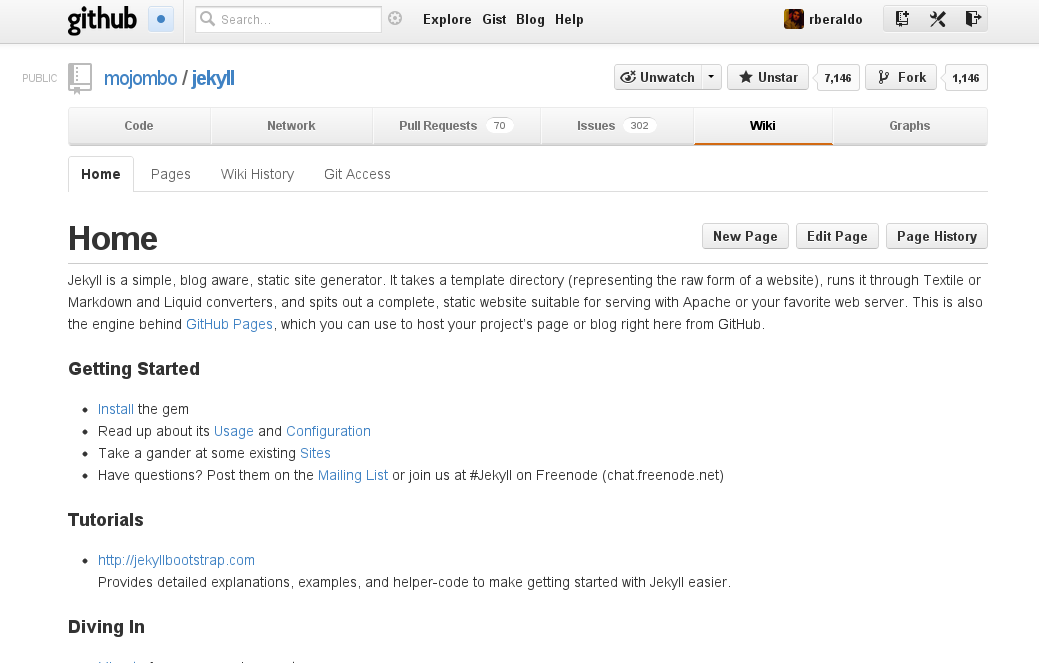
\includegraphics[width=.9\textwidth]{img/wiki.png}
  \caption{A Wiki fornecida pelo GitHub pode conter a documentação do projeto}
  \label{github:wiki}
\end{figure}

%% Imagem do bugtracker do GitHub
\begin{figure}[h]
  \centering
  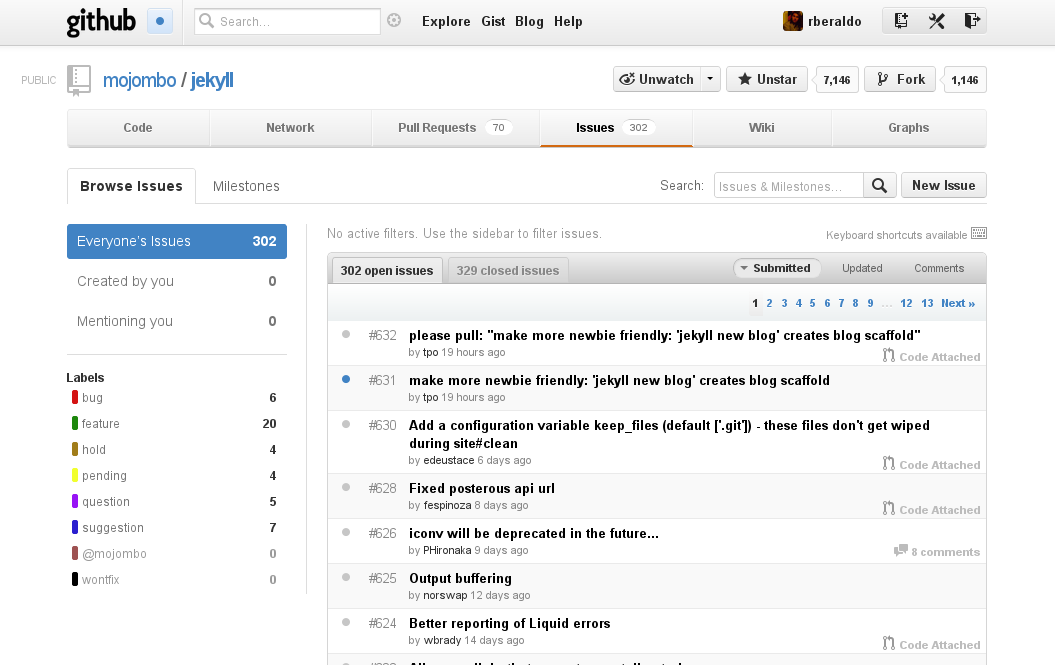
\includegraphics[width=.9\textwidth]{img/bugtracker.png}
  \caption{O \en{\textit{bug tracker}} fornecido pelo GitHub pode ajudar a resolver problemas na WordNet.Br}
  \label{github:bugtracker}
\end{figure}

A área de ajuda do GitHub\footnote{\url{https://help.github.com/}} possui uma
página explicando a configuração necessária para acessar os repositórios
disponíveis em todo o
site\footnote{\url{https://help.github.com/articles/set-up-git}}, que difere em
cada sistema operacional. A área também possui uma parte dedicada ao uso do
Git\footnote{\url{https://help.github.com/categories/19/articles}}, onde o
usuário pode encontrar referências, entre livros e vídeos, que explicam o fluxo
do trabalho usando os vários clientes disponíveis para o Git, dos mais
tradicionais, como a linha de comando, aos mais amigáveis para o usuário, como
os clientes fornecidos pelo GitHub\footnote{Cliente para Windows disponível em
\url{http://windows.github.com/} e para Mac em \url{http://mac.github.com/}}.

Com a adoção do sistema de controle de versões Git, espera-se a agilização da
construção, do armazenamento, da revisão e da atualização da base da~\wnbr\ e,
sobretudo, a sua disponibilização e as suas atualizações.
